\section{Autômatos finitos}

\begin{frame}[fragile]{Reconhecedores}

    \begin{itemize}
        \item Um reconhecedor é um programa que identifica, respondendo \code{cpp}{"Sim"} ou \code{cpp}{"Nao"}, se uma cadeia é ou não uma sentença válida de uma
            determinada linguagem
        \pause

        \item Uma estratégia para a compilação de expressões regulares em reconhecedores é o uso de diagramas de transição generalizados, denominados autômatos
            finitos
        \pause

        \item Um autômato finito pode ser determinístico ou não-determinístico: no segundo caso, podem exister duas ou mais transições com o mesmo rótulo partindo
            de um mesmo estado
        \pause

        \item Autômatos determinísticos podem resultar em reconhecimentos mais rápidos do que os não-determinísticos, porém em geral são muito maiores, no
            que diz respeito ao número de estados e transições
        \pause

        \item É possível representar expressões regulares em ambos tipos de autômatos finitos
    \end{itemize}

\end{frame}

\begin{frame}[fragile]{Autômatos finitos não-determinísticos}

    \begin{block}{Definição de AFN}
        Um autômato finito não-determinístico (AFN) é um modelo matemático que consiste em
        \begin{enumerate}
            \item um conjunto de estados $S$,

            \item um alfabeto $\Sigma$ de símbolos de entrada,

            \item uma função de transição que mapeia pares (estado, símbolo) em um conjunto de estados,

            \item um estado $s_0$, denominado estado inicial ou de partida, e

            \item um conjunto $F$ de estados de aceitação (ou estados finais).
        \end{enumerate}
    \end{block}

\end{frame}

\begin{frame}[fragile]{Grafo de transições}

    \begin{itemize}
        \item Um AFN pode ser representado por meio de um grafo direcionado e rotulado, denominado grafo de transição
        \pause

        \item Em um grafo de transição, os nós representam os estados e as arestas definem a função de transição
        \pause

        \item Os rótulos das arestas são os símbolos associados à transição, e a direção da aresta parte do estado atual para o próximo estado
        \pause

        \item Grafos de transição se assemelham aos diagramas de transição, com duas diferenças fundamentais
        \pause

        \item A primeira diferença é que um mesmo rótulo pode estar associado a duas ou mais arestas partindo de um mesmo estado
        \pause

        \item A segunda é que o símbolo \code{apl}{∊} pode rotular uma aresta
    \end{itemize}

\end{frame}

\begin{frame}[fragile]{Grafo de transição para a linguagem $(a\ |\ b)^*abb$}

    \begin{figure}
        \centering

        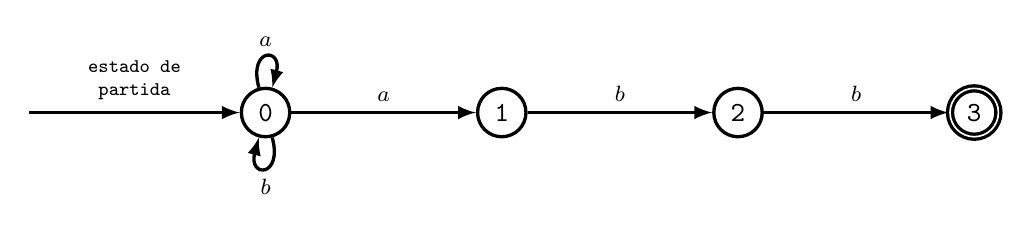
\begin{tikzpicture} 
            \coordinate (X) at (0, 6);

            \node[draw,circle,very thick] (A0) at (3, 6) { \texttt{0} };
            \node[draw,circle,very thick] (A1) at (6, 6) { \texttt{1} };
            \node[draw,circle,very thick] (A2) at (9, 6) { \texttt{2} };
            \node[draw,circle,double,very thick] (A3) at (12, 6) { \texttt{3} };

            \draw[very thick,-latex] (X) to node[above] { \scriptsize \texttt{\begin{tabular}{c}estado de\\ partida\end{tabular}} } (A0);
            \draw[very thick,-latex] (A0) to node[above] { \footnotesize $a$ } (A1);
            \draw[very thick,-latex] (A1) to node[above] { \footnotesize $b$ } (A2);
            \draw[very thick,-latex] (A2) to node[above] { \footnotesize $b$ } (A3);
            \draw[very thick,-latex] (A0) to [loop above] node[above] { \footnotesize $a$ } (A0);
            \draw[very thick,-latex] (A0) to [loop below] node[below] { \footnotesize $b$ } (A0);

        \end{tikzpicture} 
    \end{figure}
\end{frame}

\begin{frame}[fragile]{Tabela de transições}

    \begin{itemize}
        \item Uma alternativa para a implementação da função de transição é a tabela de transições
        \pause

        \item Em uma tabela de transições cada linha representa um estado e cada coluna representa um rótulo
        \pause

        \item Se necessário, é necessário adicionar uma coluna para o rótulo \code{apl}{∊}
        \pause

        \item A entrada da tabela posicionada na línha $i$, coluna $c$, contém o conjunto de estados que podem suceder o estado $i$ quando o caractere $c$
            for lido na entrada
        \pause

        \item De fato, a tabela de transições corresponde à representação do grafo de transições como uma matriz de adjacências
        \pause

        \item Outra alternativa é representar o grafo por meio de uma lista de adjacências
    \end{itemize}

\end{frame}

\begin{frame}[fragile]{Tabela de transições do AFN da linguagem $(a\ |\ b)^*abb$}

    \begin{table}
        \centering

        \begin{tabular}{ccc}
        \toprule
        \multirow{2}{*}{\textbf{Estado}} & \multicolumn{2}{c}{\textbf{Símbolo de entrada}} \\
        & $a$ & $b$ \\ 
        \midrule
        \texttt{0} & \texttt{\{ 0, 1 \}} & \texttt{\{ 0 \}} \\
        \texttt{1} & \texttt{-} & \texttt{\{ 2 \}} \\
        \texttt{2} & \texttt{-} & \texttt{\{ 3 \}} \\
        \bottomrule
        \end{tabular}
    \end{table}

\end{frame}

\begin{frame}[fragile]{Caminhos}

    \begin{itemize}
        \item Um caminho em um grafo de transições é uma sequência de arestas de transição
        \pause

        \item Os rótulos das arestas, quando concatenados, formam uma cadeia $s$
        \pause

        \item Caso o símbolo \code{apl}{∊} seja o rótulo de uma ou mais arestas de um caminho, na concatenação dos rótulos este símbolo é descartado
        \pause

        \item Um AFN aceita uma cadeia de entrada $s$ se, e somente se, existe um caminho no grafo de transições que parte do estado inicial e que termina em 
            algum estado de aceitação
        \pause

        \item Pode existir mais de um caminho que leva a um estado de aceitação
        \pause

        \item A linguagem definida por um AFN é o conjunto de cadeias que são aceitas
    \end{itemize}

\end{frame}

\begin{frame}[fragile]{AFN da linguagem $aa^*\ |\ bb^*$}

    \begin{figure}
        \centering

        \begin{tikzpicture} 
            \coordinate (X) at (0, 4);
            \node[opacity=0] (0, 0) { };

            \node[draw,circle,very thick] (A0) at (3, 4) { \texttt{0} };
            \node[draw,circle,very thick] (A1) at (6, 6) { \texttt{1} };
            \node[draw,circle,double,very thick] (A2) at (9, 6) { \texttt{2} };
            \node[draw,circle,very thick] (A3) at (6, 2) { \texttt{3} };
            \node[draw,circle,double,very thick] (A4) at (9, 2) { \texttt{4} };

            \draw[very thick,-latex] (X) to node[above] { \scriptsize \texttt{\begin{tabular}{c}estado de\\ partida\end{tabular}} } (A0);
            \draw[very thick,-latex] (A0) to node[above] { \footnotesize \code{apl}{∊} } (A1);
            \draw[very thick,-latex] (A0) to node[above] { \footnotesize \code{apl}{∊} } (A3);
            \draw[very thick,-latex] (A1) to node[above] { \footnotesize $a$ } (A2);
            \draw[very thick,-latex] (A3) to node[above] { \footnotesize $b$ } (A4);
            \draw[very thick,-latex] (A2) to [loop right] node[right] { \footnotesize $a$ } (A2);
            \draw[very thick,-latex] (A4) to [loop right] node[right] { \footnotesize $b$ } (A4);

        \end{tikzpicture} 
    \end{figure}
\end{frame}

\begin{frame}[fragile]{AFN da linguagem $aa^*\ |\ bb^*$}

    \begin{figure}
        \centering

        \begin{tikzpicture} 
            \coordinate (X) at (0, 4);
            \node[opacity=0] (0, 0) { pqgh };

            \node[draw,circle,very thick] (A0) at (3, 4) { \texttt{0} };
            \node[draw,circle,very thick] (A1) at (6, 6) { \texttt{1} };
            \node[draw,circle,double,very thick] (A2) at (9, 6) { \texttt{2} };
            \node[draw,circle,very thick] (A3) at (6, 2) { \texttt{3} };
            \node[draw,circle,double,very thick] (A4) at (9, 2) { \texttt{4} };

            \draw[very thick,-latex] (X) to node[above] { \scriptsize \texttt{\begin{tabular}{c}estado de\\ partida\end{tabular}} } (A0);
            \draw[very thick,-latex] (A0) to node[above] { \footnotesize \code{apl}{∊} } (A1);
            \draw[very thick,-latex] (A0) to node[above] { \footnotesize \code{apl}{∊} } (A3);
            \draw[very thick,-latex] (A1) to node[above] { \footnotesize $a$ } (A2);
            \draw[very thick,-latex] (A3) to node[above] { \footnotesize $b$ } (A4);
            \draw[very thick,-latex] (A2) to [loop right] node[right] { \footnotesize $a$ } (A2);
            \draw[very thick,-latex] (A4) to [loop right] node[right] { \footnotesize $b$ } (A4);

            \node[anchor=west] at (0.2, 0.2) { \footnotesize \texttt{\begin{tabular}{cc}Caminho que aceita\\ a cadeia $aa$\end{tabular}} };
            \node (B0) at (4.5, 0.2) { \footnotesize 0 };
            \node (B1) at (6.0, 0.2) { \footnotesize 1 };
            \node (B2) at (7.5, 0.2) { \footnotesize 2 };
            \node (B3) at (9.0, 0.2) { \footnotesize 2 };


            \draw[very thick,-latex] (B0) to node[above] { \footnotesize \code{apl}{∊} } (B1);
            \draw[very thick,-latex] (B1) to node[above] { \footnotesize $a$ } (B2);
            \draw[very thick,-latex] (B2) to node[above] { \footnotesize $a$ } (B3);

        \end{tikzpicture} 
    \end{figure}
\end{frame}

\begin{frame}[fragile]{Autômatos finitos determinísticos}

    \begin{block}{Definição de AFD}
        Um autômato finito deerminístico (AFD) é um caso especial de AFN no qual
        \begin{enumerate}
            \item nenhum estado possui um transição rotulada pelo símbolo \code{apl}{∊} (denominada transição-\code{apl}{∊}); e
            \item para cada estado $s$ existe no máximo uma transição rotulada com o caractere $c$ partindo de $s$.
        \end{enumerate}
    \end{block}

    \vspace{0.2in}

    \textbf{Observação}: em um AFD, cada entrada da tabela de transições contém um único estado, o que simplifica o processo de verificação de aceitação de uma cadeia.
\end{frame}

\begin{frame}[fragile]{Pseudocódigo para verificação de cadeias por meio de um AFD}

    \begin{algorithmic}[1]
        \Require{Uma cadeia de entrada $x$ terminada por um \code{cpp}{EOF}}
        \Ensure{\code{cpp}{"Sim"}, caso a cadeia seja uma sentença válida da linguagem, ou \code{cpp}{"Nao"}, caso contrário}
        \vspace{0.2in}
        \State{$s\gets s_0$}
        \State{$c\gets \Call{próximoCaractere}{\,}$}
        \Statex
        \While{$c\neq \code{cpp}{EOF}$ }
            \State{$s\gets$ \Call{transição}{$s, c$}}
            \State{$c\gets \Call{próximoCaractere}{\,}$}
        \EndWhile
        \Statex
        \If{$s\in F$}
            \State \Return{\code{cpp}{"Sim"}}
        \Else
            \State \Return{\code{cpp}{"Não"}}
        \EndIf
    \end{algorithmic}

\end{frame}

\begin{frame}[fragile]{Conversão de um AFN em um AFD}

    \begin{itemize}
        \item Dado um AFN, é possivel determinar um AFD que reconheça a mesma linguagem
        \pause

        \item A ideia central da conversão de um AFN para um AFD é fazer com que cada estado do AFD corresponda a um conjunto de estados do AFN
        \pause

        \item Seja $N$ um AFN e $D$ um AFD
        \pause

        \item O primeiro passo para a conversão é construir uma tabela de transições $Dtrans$ para $D$
        \pause

        \item Cada estado do AFD corresponderá a um conjunto de estados do AFN e $Dtrans$ será construída de forma a simular, ``em paralelo'', todas as
            possíveis transições de $N$ para uma dada entrada
        \pause

        \item Para esta tarefa, são necessárias algumas operações que envolvem um estado $s$ de $N$ e um conjunto $T$ de estados de $N$
    \end{itemize}

\end{frame}

\begin{frame}[fragile]{Operações sobre os estados de um AFN}

    \begin{table}
        \centering

        \begin{tabularx}{0.9\textwidth}{lX}
        \toprule
        \textbf{Operação} & \textbf{Descrição} \\
        \midrule
        \Call{fechamento-\code{apl}{∊}}{$s$} & Conjunto de estados do AFN atingíveis a partir do estado $s$ somente por meio de transições-\code{apl}{∊} \\
        \rowcolor[gray]{0.9}
        \Call{fechamento-\code{apl}{∊}}{$T$} & Conjunto de estados do AFN atingíveis a partir de algum estado $s\in T$ somente por meio de transições-\code{apl}{∊} \\
        \Call{movimento}{$T, a$} & Conjunto de estados do AFN para o qual existe uma transição $s\in T$ cujo rótulo é o símbolo da entrada $a$ \\
        \bottomrule
        \end{tabularx}
    \end{table}

\end{frame}

\begin{frame}[fragile]{Relação entre as operações sobre os estados de um AFN}

    \begin{itemize}
        \item Antes mesmo de ver o primeiro símbolo da entrada, $N$ pode estar em qualquer estado pertencente a \Call{fechamento-\code{apl}{∊}}{$s_0$}, onde $s_0$
            é o estado inicial
        \pause

        \item Seja $T$ o conjunto de todos os estados atingíveis a partir de $s_0$ e uma dada sequência de símbolos da entrada, e seja $a$ o próximo símbolo
        \pause

        \item Ao ver $a$, $N$ pode seguir para qualquer estado em \Call{movimento}{$T, a$}
        \pause

        \item Se existem transições-\code{apl}{∊}, $N$ pode estar em qualquer estado em \Call{fechamento-\code{apl}{∊}}{$M$}, onde $M$ = \Call{movimento}{$T, a$}, após ver $a$

    \end{itemize}

\end{frame}

\begin{frame}[fragile]{$Estados$-$D$}

    \begin{itemize}
        \item O conjunto de todos os estados de $D$ é denominado $Estados$-$D$
        \pause

        \item Cada estado de $D$ corresponde a um conjunto de estados de AFN que poderiam ser atingidos em $N$ após uma sequência de símbolos da entrada, incluindo
            as possíveis transições-\code{apl}{∊} antes ou depois dos símbolos serem vistos
        \pause

        \item O estado de partida de $D$ é \Call{fechamento-\code{apl}{∊}}{$s_0$}
        \pause

        \item Os demais estados são adicionados segundo o algoritmo descrito a seguir
        \pause

        \item Os estados de aceitação de $D$ são aqueles cujo conjunto de estados de AFN que representa contém ao menos um estado de aceitação de $N$
    \end{itemize}

\end{frame}

\begin{frame}[fragile]{Construção de subconjuntos}

    \begin{algorithmic}[1]
        \State{$F\gets \Call{fechamento-\code{apl}{∊}}{s_0}$}
        \State{Desmarque $F$}
        \State{Inclua em $F$ em $Estados$-$D$}
        \While{existe um estado $T\in Estados$-$D$ não marcado}
            \State{Marque $T$}
            \For{cada símbolo de entrada $a$}
                \State{$M\gets \Call{movimento}{T, a}$}
                \State{$U\gets \Call{fechamento-\code{apl}{∊}}{M}$}
                \If{$U\not\in Estados$-$D$}
                    \State{Desmarque $U$}
                    \State{Inclua $U$ em $Estados$-$D$}
                \EndIf
                \State{$Dtrans[T, a]\gets U$}
            \EndFor
        \EndWhile
    \end{algorithmic}

\end{frame}

\begin{frame}[fragile]{Cálculo de \Call{fechamento-\code{apl}{∊}}{$T$}}

    \begin{algorithmic}[1]
        \State{Seja $P$ uma pilha}
        \State{Empilhe em $P$ todos os estados em $T$}
        \State{Inclua $T$ em \Call{fechamento-\code{apl}{∊}}{$T$}}
        \While{$P$ não estiver vazia}
            \State{Desempilhe o topo $t$ de $P$}
            \For{cada estado $u$ que é chegada de uma aresta partindo de $t$ com rótulo \code{apl}{∊}}
                \If{$u\not\in$ \Call{fechamento-\code{apl}{∊}}{$T$}}
                    \State{Inclua $u$ em \Call{fechamento-\code{apl}{∊}}{$T$}}
                    \State{Empilhe $u$}
                \EndIf
            \EndFor
        \EndWhile
    \end{algorithmic}

\end{frame}

\begin{frame}[fragile]{AFN para a linguagem $(a\ |\ b)^*abb$}

    \begin{figure}
        \centering

        \begin{footnotesize}
        \begin{tikzpicture} 
            \coordinate (X) at (0, 3);

            \node[draw,thick,circle] (A0) at (2, 3) { \texttt{0} };
            \node[draw,thick,circle] (A1) at (4, 3) { \texttt{1} };
            \node[draw,thick,circle] (A2) at (5, 5) { \texttt{2} };
            \node[draw,thick,circle] (A3) at (7, 5) { \texttt{3} };
            \node[draw,thick,circle] (A4) at (5, 1) { \texttt{4} };
            \node[draw,thick,circle] (A5) at (7, 1) { \texttt{5} };
            \node[draw,thick,circle] (A6) at (8, 3) { \texttt{6} };
            \node[draw,thick,circle] (A7) at (10, 3) { \texttt{7} };
            \node[draw,thick,circle] (A8) at (12, 5) { \texttt{8} };
            \node[draw,thick,circle] (A9) at (12, 3) { \texttt{9} };
            \node[draw,thick,circle,double] (A10) at (12, 1) { \texttt{10} };

            \draw[thick,-latex] (X) to node[above]{ \begin{tabular}{c}\texttt{estado}\\ \texttt{inicial}\end{tabular} } (A0);
            \draw[thick,-latex] (A0) to node[above]{ \code{apl}{∊} } (A1);
            \draw[thick,-latex] (A1) to node[above left]{ \code{apl}{∊} } (A2);
            \draw[thick,-latex] (A2) to node[above]{ $a$ } (A3);
            \draw[thick,-latex] (A1) to node[below left]{ \code{apl}{∊} } (A4);
            \draw[thick,-latex] (A4) to node[below]{ $b$ } (A5);
            \draw[thick,-latex] (A3) to node[above right]{ \code{apl}{∊} } (A6);
            \draw[thick,-latex] (A5) to node[below right]{ \code{apl}{∊} } (A6);
            \draw[thick,-latex] (A6) to node[above]{ \code{apl}{∊} } (A7);
            \draw[thick,-latex] (A7) to node[above left]{ $a$ } (A8);
            \draw[thick,-latex] (A8) to node[left]{ $b$ } (A9);
            \draw[thick,-latex] (A9) to node[left]{ $b$ } (A10);
            \draw[thick,-latex] (A0) to [bend right=100] node[below]{ \code{apl}{∊} } (A7);
            \draw[thick,-latex] (A1) to [bend left=30] node[above]{ \code{apl}{∊} } (A6);

        \end{tikzpicture} 
        \end{footnotesize}
    \end{figure}

\end{frame}

\begin{frame}[fragile]{Convertendo o AFN em um AFD}

    \begin{itemize}
        \item O estado inicial do AFD será o estado
        \[
            \texttt{A} = \Call{fechamento-\code{apl}{∊}}{\texttt{0}} = \{ \texttt{0, 1, 2, 4, 7} \}
        \] \pause

        \item Veja que no cálculo de \Call{fechamento-\code{apl}{∊}}{\texttt{0}}, o estado \texttt{0} é atingível por meio de um caminho vazio
        \pause

        \item O alfabeto da linguagem é $\Sigma = \{\ a, b\ \}$
        \pause

        \item Seguindo o algoritmo, o próximo estado será \texttt{B} = \Call{fechamento-\code{apl}{∊}}{$M$}, onde $M$ = \Call{movimento}{$A, a$}
        \pause

        \item Segue que
        \[
            M = \Call{movimento}{A, a} = \Call{movimento}{\{\texttt{0, 1, 2, 4, 7}\}, a} = \{\texttt{3, 8}\} 
        \]
    \end{itemize}

\end{frame}

\begin{frame}[fragile]{Convertendo o AFN em um AFD}

    \begin{itemize}
        \item Daí
        \[
            \texttt{B} = 
                \Call{fechamento-\code{apl}{∊}}{\{\texttt{3, 8}\}} =  \{\texttt{1, 2, 3, 4, 6, 7, 8}\}
        \]
        \pause

        \item A transição entre estes dois estados deve ser registrada na tabela $Dtrans$:
        \[
            Dtrans[\texttt{A}, a] = \texttt{B}
        \]
        \pause

        \item O próximo estado \texttt{C} é computado a partir de \Call{movimento}{\texttt{A}, $b$} $= \{\texttt{5}\}$:
        \[
             \texttt{C} = \Call{fechamento-\code{apl}{∊}}{\{\texttt{5}\}} =  \{\texttt{1, 2, 4, 5, 6, 7}\}
        \]
    \end{itemize}

\end{frame}

\begin{frame}[fragile]{Convertendo o AFN em um AFD}

    \begin{itemize}
        \item Assim, $Dtrans[\texttt{A}, b] = \texttt{C}$
        \pause

        \item Seguindo o algoritmo, apenas mais dois estados distintos serão encontrado:
        \[
            \begin{array}{l}
                \texttt{D} = \{\texttt{1, 2, 4, 5, 6, 7, 9}\} \\
                \texttt{E} = \{\texttt{1, 2, 4, 5, 6, 7, 10}\} \\
            \end{array}
        \]
        \pause

        \item Dentre os estados identificados, apenas \texttt{E} é estado de aceitação, pois contém o estado \texttt{10} de $N$
        \pause

        \item No pior caso, seriam identificados $2^n$ novos estados, onde $n$ é o número de estados do AFN
    \end{itemize}

\end{frame}

\begin{frame}[fragile]{Resultado da conversão do AFN para um AFD}

    \begin{figure}
        \centering

        \begin{footnotesize}
        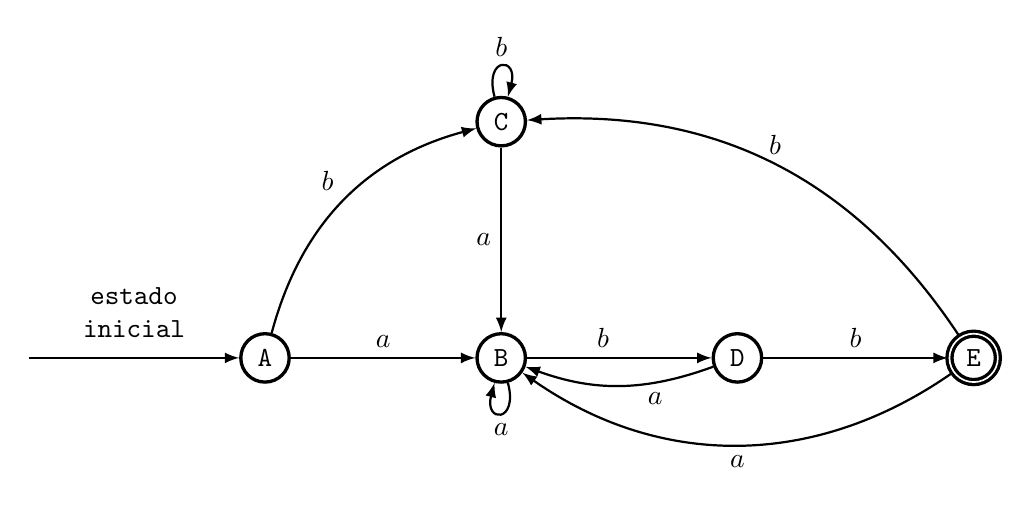
\begin{tikzpicture} 
            \coordinate (X) at (0, 3);

            \node[draw,very thick,circle] (A) at (3, 3) { \texttt{A} };
            \node[draw,very thick,circle] (B) at (6, 3) { \texttt{B} };
            \node[draw,very thick,circle] (C) at (6, 6) { \texttt{C} };
            \node[draw,very thick,circle] (D) at (9, 3) { \texttt{D} };
            \node[draw,very thick,circle,double] (E) at (12, 3) { \texttt{E} };

            \draw[thick,-latex] (X) to node[above]{ \begin{tabular}{c}\texttt{estado}\\ \texttt{inicial}\end{tabular} } (A);
            \draw[thick,-latex] (A) to node[above]{ $a$ } (B);
            \draw[thick,-latex] (A) to [bend left] node[above left]{ $b$ } (C);
            \draw[thick,-latex] (B) to [loop below] node[below]{ $a$ } (B);
            \draw[thick,-latex] (B) to node[above left]{ $b$ } (D);
            \draw[thick,-latex] (C) to node[left]{ $a$ } (B);
            \draw[thick,-latex] (C) to [loop above] node[above]{ $b$ } (C);
            \draw[thick,-latex] (D) to [bend left=20] node[below,pos=0.3]{ $a$ } (B);
            \draw[thick,-latex] (D) to node[above]{ $b$ } (E);
            \draw[thick,-latex] (E) to [bend left=35] node[below]{ $a$ } (B);
            \draw[thick,-latex] (E) to [bend right] node[above]{ $b$ } (C);

        \end{tikzpicture} 
        \end{footnotesize}
    \end{figure}

\end{frame}


